\pagebreak
\section{Results}
\add[XT]{add one more section as an individual file/chapter for 2D models description.}
\subsection{3D model results}
%\add[XT]{choose some points in the model domain like Choi 2008 did, to monitor the values changes with time (e.g. In VisIt use Query to obtain stress with time for quantatatively analyzing the model behaviors)}
\note[EC]{This paragraph would fit better in the ``Parameters to Control'' section.} \change[EC]{Currently, we}{I} have three factors controlling the model behaviors. They are three ranges of M variation along the ridge axis (0.5$\sim$0.7; 0.5$\sim$0.8; 0.2$\sim$0.8), three functional forms of M variation (linear; sinusoidal; square root) and two types of weakening rate (Type 1 and Type 2)\remove[EC]{ as described in detail in the section ``Parameters to control''}. 

Generally, all models forms a median valley that deepens and widens toward the lower M side except the reference model with constant M $=0.8$. The topography oberseved in our models, to the first order, is controlled by the spatial and temporal distributions of faulting and to the second order, results from elastic\remove[EC]{ally} deformation\add[EC]{s} \change[EC]{(e.g. T}{such as t}he gradual deepening and widening of the median valley\change[EC]{; T}{and t}he bending of the crust at the footwall side of the detatchment fault results in a domal shape of the fault interface as a mechanism for producing the dome shape of OCCs).\note[EC]{I think these processes are more than elastic deformations. Think again about the validity of the last sentence.}

The pattern of the deformation (faulting and elastic deformation) is controlled by the evolving stress in the crust in terms of its distribution and magnitude. The stress evolution is a result of the interaction processes between tectonics and magmatism. Due to constant seafloor spreading, tensional stress orthogonal to the ridge-axis in the crust keeps accummulating. At the same time, along ridge-axis varying diking partially accommodates the stress from far field extension and perturbs the homogeneity state of stress distribution along the ridge-axis. Accumulated stress will be largely released when the normal or shear failures establish.\add[EC]{This paragraph is almost like notes to yourself. Too general to be called a result.}

In this ``Results'' chapter, we will first focus on describing model behaviors in detail of two reference models and base on that, we will compare the reference model and the other data points with different setup parameters. Formation mechanism will be explained for part of the the model behaviors in this chapter and will be further discussed in ``Discussion'' chapter. 

\subsection{Reference model description\note[EC]{Isn't this supposed to be a subsubsection since it's a part of the 3D model results?}}
We consider \annote[EC]{two models as our reference models}{Usually, if not necessarily, we take only one model as a reference.}: one, M varies linearly from 0.2 to 0.8 along the ridge axis with increasing Z; two, constant M along the ridge axis as a comparison to the changing M models.

\subsubsection{M varies along the ridge axis\note[EC]{}

\begin{figure}[hc]
  \centering
    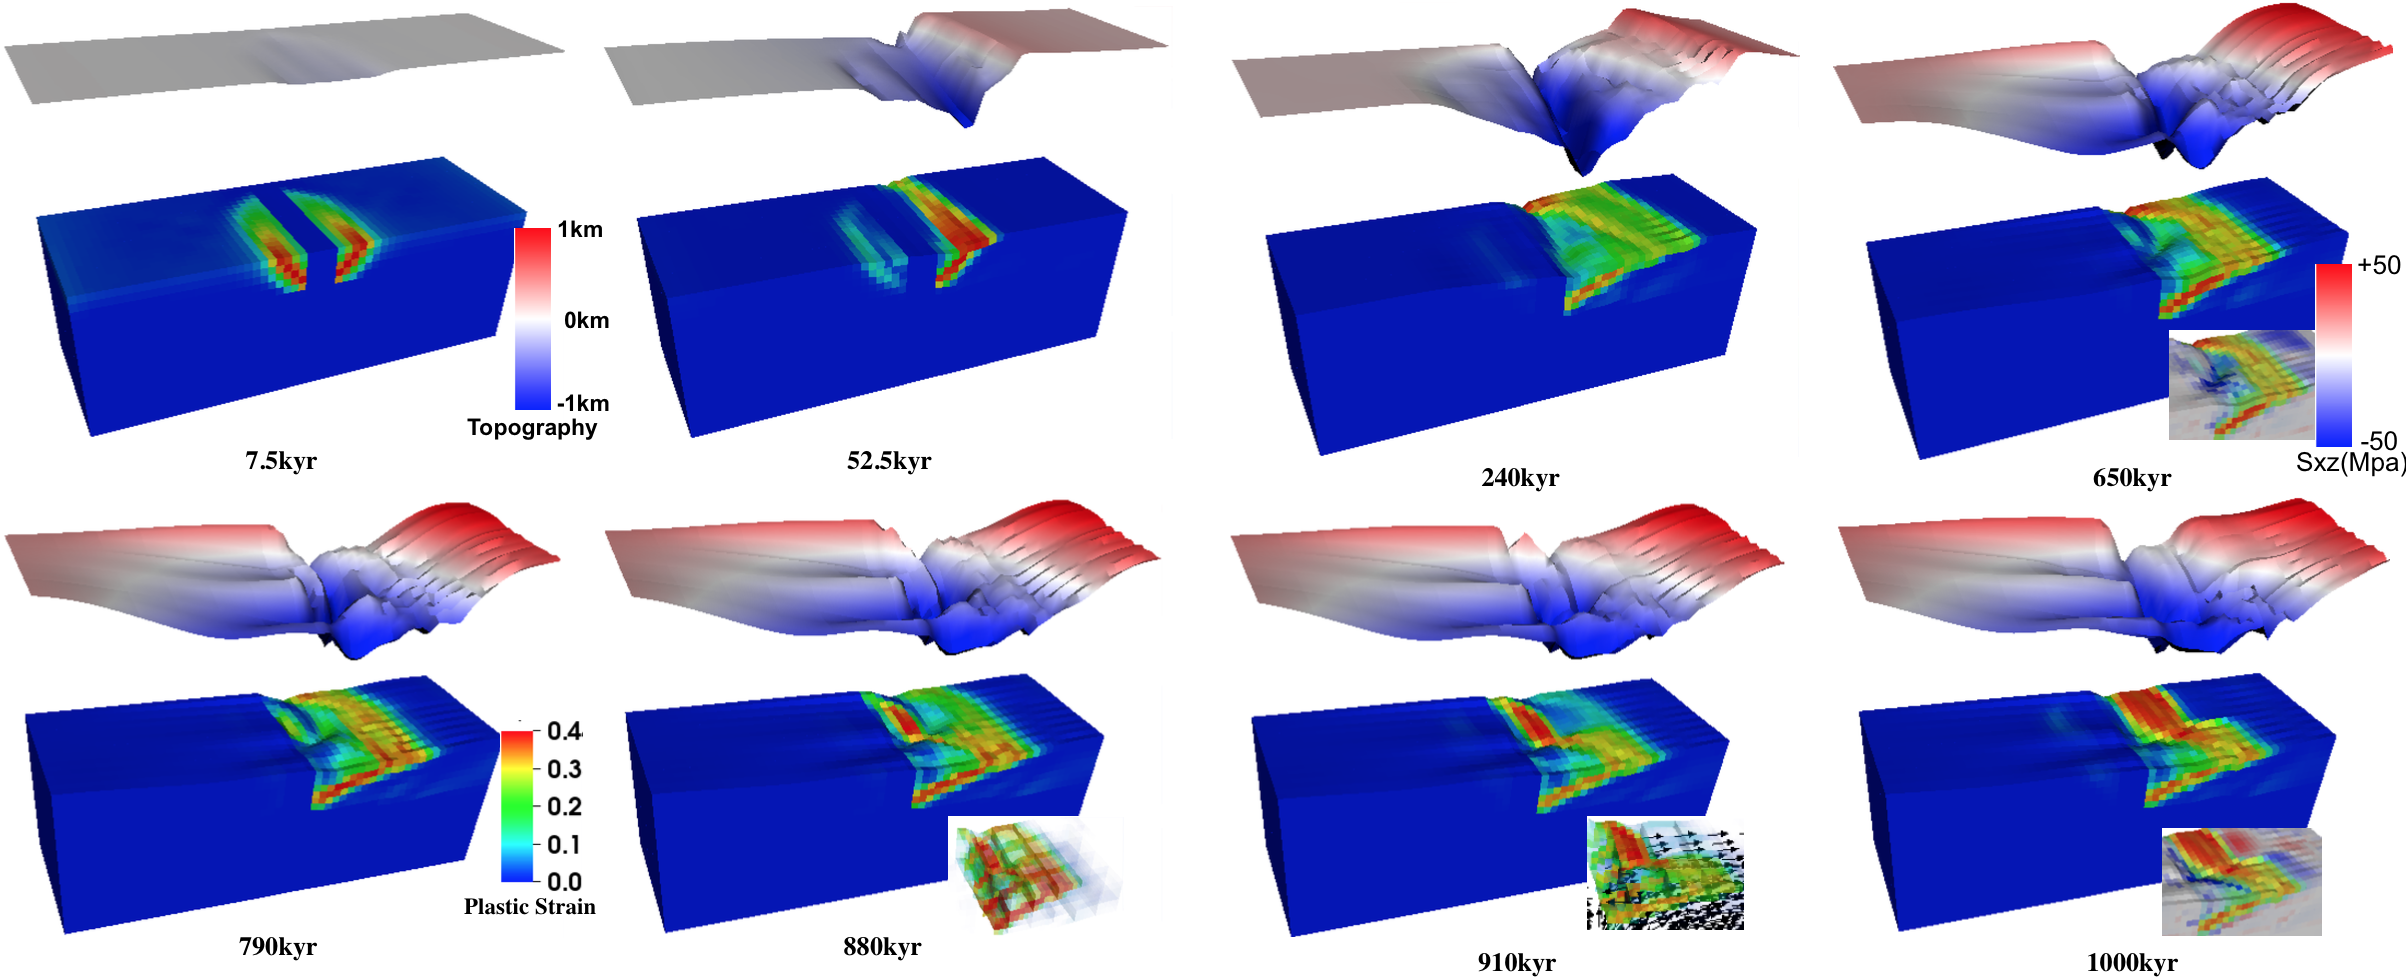
\includegraphics[width=1.0\textwidth]{fig_Results1_1.png}
  \caption{Reference model one: M linearly increases from 0.2 to 0.8 from front to back. The top layer is the topography of the model with five times vertical exaggeration. The color scale within Figure~\ref{fig_Results1_1}.a is for the topography. Initial seafloor is marked as a reference of zero km in height.  The green, yellow and red colors in the background of blue model domain are plastic strain. Its color scale is shown in Figure~\ref{fig_Results1_1}.e. The number with kyr as a unit beneath each model result is the time for the model with a unit of thousands of year. The two insets in Figure~\ref{fig_Results1_1}.b and Figure~\ref{fig_Results1_1}.d is for stress $\sigma_{xx}$ (Sxx in the figure). Positive value (pink and red) means tension and negative (blue) is compression. The inset in Figure~\ref{fig_Results1_1}.h is for shear stress $\sigma_{xz}$ (Sxz in the figure). It share the same color scale with insets in the Figure~\ref{fig_Results1_1}.b and Figure~\ref{fig_Results1_1}.d. The inset in Figure~\ref{fig_Results1_1}.f is a transparent view of plastic strain. The inset in Figure~\ref{fig_Results1_1}.g shows both plastic strain and the velocity vector. Indicated by the velocity vector, the hanging wall of the detachment fault at low M region (M0.2$\sim$M0.5) is moving in an opposite direction to the hanging wall at higher M region (M$>0.5$).} %\note[XT]{one thing to be noted is that the $dt=0.5yr$ in these series of 3D models, thus I divided the time step by two to get the time (kyr). This figure needs to be revised that the plastic strain scale is actually changing for different time, a way to revise it is to maintain a constant color scale or attach a color scale for each time. Also, it seems a little bit small and two rows is not as preferable as one row or one column to better express the concept of linear time series evolution.}}
 \label{fig_Results1_1}
\end{figure}   

As shown in Figure~\ref{fig_Results1_1}, the model create\add[EC]{s} a median valley that both widens and deepens through time and the rate of its widening and deepening at a specific location (in terms of Z-axis) is inverse\add[EC]{ly} proportional to the rate of local magma supply (i.e. M value). Kilometers in relief and tens of kilometers in lentgh OCCs are produced in the model. One interesting behavior worth noting is that corrugations with hundred-to-kilometer wavelengths are also produced by the model.\note[EC]{Looks like this first paragraph is an overview

As shown in Figure~\ref{fig_Results1_1}.a, in the first 7.5kyr, high angle ($\sim 60 \degree$)(consistent with  Anderson's theory of faulting mechanics for a frictional angle of 30$\degree$) normal faults (shown as higher plastic strain shear bands with a thickness of 2$\sim$4 times of the width of a single hexahedron element) begin to form near the ridge axis in terms of plastic strain localization near the ridge center (weakest place to deform), because of the thickness of the crust is thinnest at the ridge center due to our thermal structure setup. For each timestep, the tensional stress accummulates faster at the lower M side where the crust reaches a yielding point earlier than higher M side and so the fault first initiate at the front (lower M side) and then propagates to the back (higher M side). However, the along ridge-axis coupling (internal strength preventing relative displacement (i.e. rotation, offset) between two neighbors along the Z-axis) assists in fault propagation from front to back and reduces the time difference in initiation of faulting along the ridge-axis \annote[XT]{when comparing with separate 2D models}{It probably will be verified after a 2D results analysis and conclusion}.  

At 52.5kyr (Figure~\ref{fig_Results1_1}.b), the normal fault on the right hand side of the ridge axis continues to evolve while the one on the left becomes inactive. The choice of which fault will delvelop is a random event since the model setup is symmetrical across the ridge-axis. The timing difference of initiation of faulting along the ridge axis creates an offset in X-axis direction between along ridge-axis breakways that the breakaway at the lower M side extends further than that of the higher M side (Figure~\ref{fig_Results1_4}). This offset remains constantly around three elements until time 295kyr (Figure~\ref{fig_Results1_4}.d) because the extending velocity of the breakaway to move away from the ridge-axis is only controlled by the far field extension rate, $V_{x}$. \add[XT]{Why after 295kyr the offset reduces needs to be answered. I don't know now. Probably partly due to healing that earlier the fault initiation, more healing it experiences.} In addition, as shown in the inset of $\sigma_{xx}$, as the fault offsets, crust at the footwall begins to bend in a clockwise rotation (view from front) and the neutral plane ($\sigma_{xx}=0$) is shown as the boundary between blue (compression) and pink (tension). In the ``Discussion'' section, we will show that this bending force created in the crust of footwall is essential for major faulting evolution.
%the fault displacement at the front side is larger than that of the back because M is lower at the front and more extension needed to be accommodated by the tectonic processes (i.e. normal faulting). \annote[XT]{Thus, the breakaway at the front extending further away from the ridge axis.}{I am not sure whether the breakaway extends further at lower M side because it should be the same. The breakaway at lower M side does extend further not because of fault slip rate difference but becauses of initiation time, at lower M side, fault begin earlier thus the breakaway begin to extend earlier and reach further, however, the rate of extending away from axis for the breakway should equal to the extension rate $V_{x}$. Thus the offset between breakaways of front and back remains constant} The termination of the detachment fault where footwall begins to be exhumed to the surface will extend further due of faster bending of the footwall at the lower M side. This will also result in a larger volume of exhumation at the lower M side than that of the higher M side. For our model that even when $M=0.2$, the detachment fault can still last for a long time \citep{Baines2008}, the exhumation rate has a upper limit of extension rate of $V_{x}$ in spite of a higher fault slip rate at lower M side.  


The location of the termination of the detachment fault where footwall begins to be exhumed to the surface varies along the ridge-axis (i.e. Z-axis). As shown in Figure~\ref{fig_Results1_2}, the highest strain rate regions (red) can be interpreted as detachment fault interfaces. When M$<=0.5$, although the rate of fault slip should be higher for lower M, the rate of bending or decreasing in dip angle of the fault has a maximum value corresponds to the far field extension rate. Because for M$<0.5$, the detachments root at the same place (center dike at a depth five to six elements beneath the surface)(Figure~\ref{fig_Results1_2}.Z=0, 5, 10) along the ridge-axis, the amount of bending in the footwall of the detachment is determined by the amount of the displacement of the breakaway. In other words, because in order to spend least frictional energy during faulting, fault interface between the two ends tends to be a straight line. Thus, the dip angle of the fault is inverse proportional to the distance between the breakaway and the root of the normal fault when M$<0.5$. So the further between the breakaway and the root of the fault, the lower its dip angle. Since the breakaways at the region with M$<0.5$ is pulled with the same velocity $V_{x}$, the distances between the breakaways and the roots of the faults are the same. Thus the dip angles of the faults at the same time along the ridge-axis are the same. However, when M$>0.5$, the amount of fault slip decreases as M increase and the crust at the footwall experiences less bending and the detachment remains in high angle with closer to ridge-axis termination (Figure~\ref{fig_Results1_2}.Z=15, 20). This is due to the root of the fault is being slowly pushed away from ridge-axis while the breakaway of the fault is closer to ridge center since the fault initiates later than that at the low M side. In addition, the crust thickness the fault cut through is slowly increasing as the fault being pushed away from ridge center due to excessive diking. These three factors together contribute to a higher dip angle. In a unit time, the volume of the exhumation is also smaller for the higher M side. One thing needs to be noted that the lowest topography points at high M side correspond to the terminations but detached from the terminations at the low M side (M$<0.5$) as shown in Figure~\ref{fig_Results1_2}.        

\begin{figure}[hc]
  \centering
    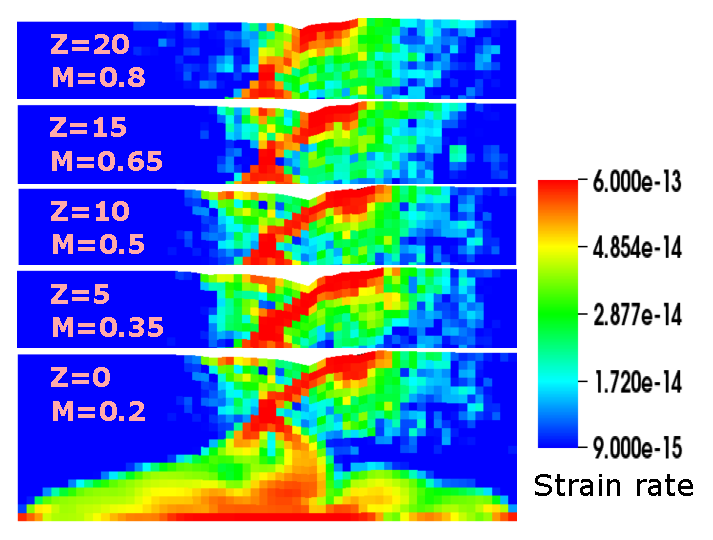
\includegraphics[width=0.6\textwidth]{fig_Results1_2.eps}
  \caption{Strain rate at 107.5kyr with five slices along ridge axis(Z axis).}
 \label{fig_Results1_2}
\end{figure}   

\begin{figure}[hc]
  \centering
    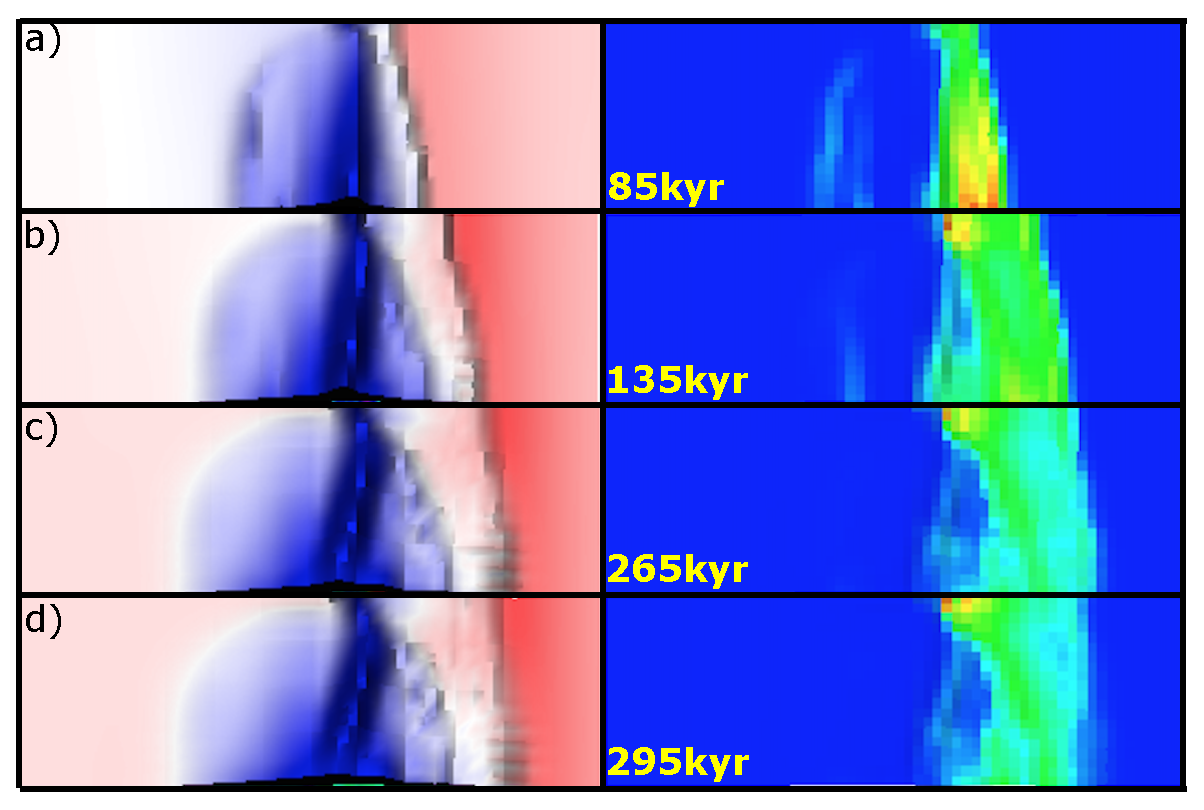
\includegraphics[width=0.6\textwidth]{fig_Results1_4.eps}
  \caption{Breakaway evolution through time. Viewing from top. Left column is topography at different time; Right column is plastic strain. They both share same color scales in the figure~\ref{fig_Results1_1}. The offset between breakways along the ridge-axis in X-axis direction remains three elements until time 295kyr. It also shows that the lowest topography points along the ridge-axis start as a straigt line parellel with ridge-axis in a) and then gradually become oblique to the ridge-axis. Please see text for detail description.}
 \label{fig_Results1_4}
\end{figure}

At 240kyr (Figure~\ref{fig_Results1_1}.c), the median valley further deepens and widens. The detachment keeps active and extends to $\sim$18km in length horizontally (longest at M$=0.2$) with the dip angle decreases from initially $\sim$60$\degree$ to 30$\degree$(at the root of the fault) and 0$\degree$ where the fault interface is exposed to the seafloor. However, for the detachment at the higher M side (especially the last three elements along the Z-axis), the dip angle remains high. The maximum relief between highest point in breakaway and lowest point in the median valley becomes larger than 1km. Corrugations show up at the lower M side, at the front tip of the extending fault interface. The lowest topography points inside the median valley evolves from a straight line parallel to the ridge-axis (Figure~\ref{fig_Results1_4}.a) to a line oblique to the ridge-axis (Figure~\ref{fig_Results1_4}.b,c,d). Initially, the lowest topography points are at the terminations of the detachment fault. Due to the coupling along the ridge-axis, fault propagates from front to back in a straight line parallel to the ridge-axis. However, as the dip angle of the detachment at the low M side begin to decrease due to bending of the crust at the footwall, along with excessive tensional stress result from low magma supply, the lowest topography point at the lower M side is pulled to the conjugate plate. While the lowest topography points at the high M side (M$>0.5$) are pushed away from the dike. Note that the oblique lowest topography points form not a straight line, but a curve that the lowest point remains near axis at the high M side. This is due to the bending rate of the detachment at high M side is very low and thus the termination can remains near the ridge-axis.      
%{Important tecnique from discussion on Mar. 9th with Eunseo: 1. One way to analyze models is to make hypothesis to describe model behaviors and than use models to approve or reject it. If rejected, find a new hypothesis and do the same thing again.}
%\add[XT]{4. An new thinking on little termination or dip angle variation when M$<0.5$ as observed in %figure~\ref{fig_Results1_2}: why along-z hanging wall has little variation is because we have along z coupling, the rotational shear failure between along-z neighbors are so hard. and also, the more extension in M0.2 end is accommodated elastically by the whole plate to the left of the detachment fault which can be observed as lower topo(topography variation along ridge axis).} 

\add[XT]{One question needs to be answered: at 410 timesteps (205kyr), the breakaway at the front already extends 15km, assumming a constant extending rate, it means a velocity of around 75km/Myr, much faster than half spreading rate 25km/Myr. If it is true, I need to change previous discussion on how fast breakaway being pulled away from ridge-axis.}

At 650kyr (Figure~\ref{fig_Results1_1}.d), the median valley continues to deepen and widen. The breakaways along the ridge-axis already \annote[XT]{moved out of the model domain}{it should not, if breakaway move with 25km/yr(half spreading rate), since the distance between initial break (5km away from ridge center) and right wall of the model domain is about 25km which needs 1Myr to reach. But now is only 650kyr. Why is it?}. The fault offset is already larger than the thickness of the crust and the upper mantle materials begin to be exhumed to the surface. The previous fault interface bend over to a negative dip angle (dip in an opposite direction) and produces a dome shape OCC with corrugations on its surface parallel to the spreading direction. The previous lowest topography points evolve to a curve with bigger curvature. Compared to the inset in Figure~\ref{fig_Results1_1}.b, the total length of the bending crust decreases. A hint of a near-axis secondary fault begin to initial at the high M side ($10<$Z$<15$) as a form of tension failure. \add[XT]{Its formation will be discussed in Discussion section accompanied by the stress status analysis. }

At 790kyr (Figure~\ref{fig_Results1_1}.e), the initial tension failure immediately ajacent to the ridge center (hint of the secondary fault) begin to evolve and propagate to higher Z region.  

At 880kyr (Figure~\ref{fig_Results1_1}.f), at the higher M side, the initial tension failure evolves to a high angle near-axis secondary normal fault and replace the initial detachment as indicated in the inset of transparent view of plastic strain.

At 910kyr (Figure~\ref{fig_Results1_1}.g), the secondary normal fault results in a strong constrast in moving directions between high M side and low M side near the ridge-axis that at the high M side, previous hanging wall becomes footwall and moves with spreading direction on the right, however, at the low M side, due to deficit in magma supply, hanging wall is coupled with conjugate plate and move to the left as shown in the inset. This opposite direction motion creates a strong shear stress region $\sim$45$\degree$ oblique to the ridge-axis (inset of Figure~\ref{fig_Results1_1}.h) and produces new lowest topography points align with it. Combined with previous lowest topography points, an ``X'' shape topography low is created.

Corrugations are observed in the model since 240kyr. It will be further discussed in the discussion chapter. There are two contributing factors, for one, trans-extenstional stresses are created due to offset of the breakaway as well as the variation in fault displacements along the ridge axis; for the other, the variation of the positions of the terminations of the detachment faults along the ridge-axis creates anastomosing faults that is mentioned in \citep{Smith2014}. This anastomosing faulting behavior is largely responsible for corrugations in our models.      

\subsubsection{Constant M along the ridge axis }
Another reference model is the model with constant M$=0.8$ along the ridge axis as a comparison to the changing M models.

As shown in Figure~\ref{fig_Results1_3}, this constant M along the ridge-axis model create a median valley of $\sim 20km$ in width and $1\sim2km$ in depth which is similar to generally observation of Mid-Atlantic Ridges. The width and depth of the median valley is almost constant along the ridge-axis. The variation along the ridge-axis in breakaway and termination as well as the existence of corrugation mentioned in reference model one are not observed. 
\begin{figure}[hc]
  \centering
    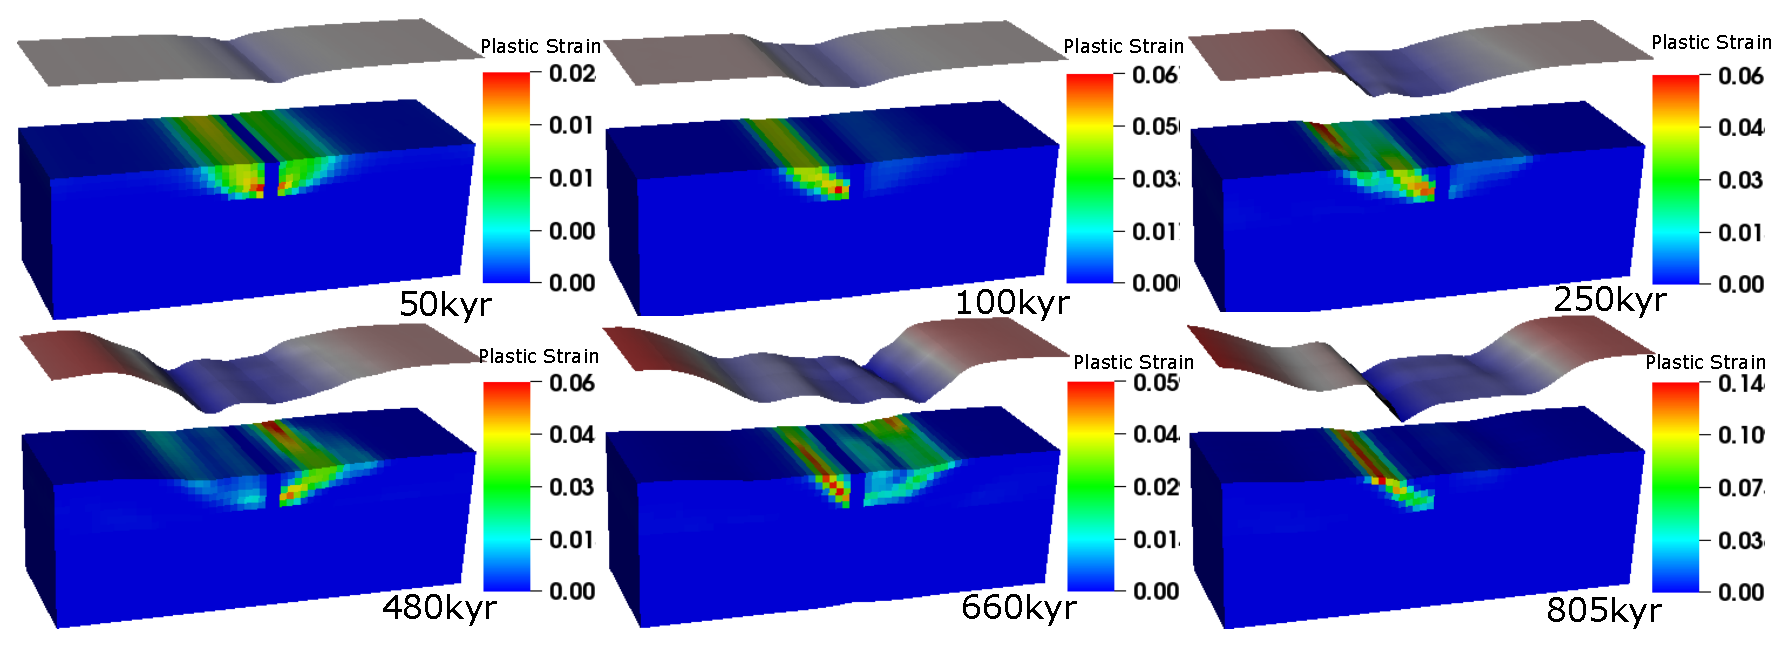
\includegraphics[width=1.0\textwidth]{fig_Results1_3.eps}
  \caption{Reference model two: constant M$=0.8$ along the ridge-axis (i.e. Z axis). Type two weakening.}
 \label{fig_Results1_3}
\end{figure}   

Based on the previous experience in pseudo-2D models or \citep{Lavier2000}, with higher characteristic fault offset ($\Delta X_{c}$) for Type two weakening compared with Type one weakening, the frequency of normal faulting alternation is higher for M$>0.5$ cases. However, interesting enough, when comparing pseudo-2D and 3D models when they are using Type two weakening under case of M$=0.8$, even though the 3D Model has a larger $\Delta X_{c}$ of 1km than that of pseudo-2D model of 0.5kmr, 3D model has a lower frequency of faulting alternation. Since M is constant 0.8 along the ridge-axis, the effect of along ridge couplingthat resists alternation need not be considered. One possibility is that the resisting bending force increase in a higher rate than linear with respect to increasing the length of the ridge segment (Z$_{max}$ km).  

\subsection{Tables of all the data points}

Currently, we have run \annote[XT]{hundreds of}{find out exactly number that will be used in 2D model results conclusion} Psedudo-2D models for initial setup and benchmarking with previous studies (e.g. \citep{Buck2005} and \citep{Tucholke2008}). Based on those Pseudo-2D models, we further ran 11 3D models. The available data points are limited due to the huge computation expenses for 3D models (For each model to be run to 2Myr, usually needs 192 cores for about 2 days (around 10000 SUs). \add[XT]{use 96 cores can improve the efficiency a little bit (Longer time but smaller amount of SUs needed).})

\begin{table}[H]
\begin{small}
\begin{center}
\begin{tabular}{||l|l||l|l||l|l||}
\hline
A & Alternating Fault & C & Corrugation & SL & Shear Topography Low \\
\hline
NA& Not Alternating & SF & Secondary Fault on one side & CB & Cut Back   \\
\hline
DD &  Double Dome  & AM    & Atlantis Massif &  &   \\
\hline
\end{tabular}
\end{center}
\end{small}
\caption{Model behaviors in short.}
\label{Tab1}
\end{table}

Based on the 11 models, we observed eight first-order behaviors as shown in Table~\ref{Tab1}. 

\begin{table}[H]
\begin{small}
\begin{center}
\begin{tabular}{|l|p{3.5cm}|p{3.5cm}|p{3.5cm}|}
\hline
\diagbox[width=12em]{Weakening type}{M range}&
M28&M57&M58\\
\hline
Type one &NA; C; SL; SF$_{1500kyr}$; DD    &NA; C; SF$_{1380kyr}$; CB$_{330kyr}$; AM(opposite z)     &    \\
\hline
Type two &    &     &    \\
\hline
\end{tabular}
\end{center}
\end{small}
\caption{Linear functional form.}
\end{table}

\begin{center}
\begin{table}[H]
\begin{small}
\begin{tabular}{|l|p{3.5cm}|p{3.5cm}|p{3.5cm}|}
\hline
\diagbox[width=12em]{Weakening type}{M range}&
M28&M57&M58\\
\hline
Type one & NA; C; SL; SF$_{995kyr}$ & NA; C; SL; SF$_{760kyr;1320kyr}$; CB$_{520kyr}$; AM & NA; C; SL; CB$_{510kyr}$; SF$_{760kyr;1140kyr;1990kyr}$   \\
\hline
Type two &    &NA; C; SL; SF$_{680kyr}$; CB$_{905kyr}$     & A$_{450kyr;600kyr}$; C(only at low M); CB$_{990kyr}$   \\
\hline
\end{tabular}
\end{small}
\caption{Sinusoidal functional form.}
\end{table}
\end{center}

\begin{table}[H]
\begin{small}
\begin{center}
\begin{tabular}{|l|p{3.5cm}|p{3.5cm}|p{3.5cm}|}
\hline
\diagbox[width=12em]{Weakening type}{M range}&
M28&M57&M58\\
\hline
Type one & NA; C; SL; CB$_{205kyr;330kyr;1025kyr}$   &      & NA; C$_{1770kyr}$(due to shear with dif wave length); SF$_{860kyr}$(high M); SF$_{1190kyr}$(low M)(Dog Bone); SF$_{1690kyr}$    \\
\hline
Type two &    & NA; C; SF$_{435kyr;1060kyr}$; CB$_{585kyr}$; CB$_{735kyr}$; CB$_{910kyr}$; CB$_{970kyr}$    & A$_{550kyr;920kyr}$; C; CB$_{400kyr}$    \\
\hline
\end{tabular}
\end{center}
\end{small}
\caption{Square root functional form.}
\end{table}

Based on the available data points as shown in the tables, we are able to compare the model results with respect to three factors: 1) Variation of the range of M; 2) Variation of the functional form and 3) Influence of weakening rate. 

\subsection{Variation of the functional form}
How magma supply varies along the MORs ridge-axis remains a current research question and we do not have direct quantitative observation over it. However, from indirect geophysical studies (e.g. gravity, seismology), people suggest a general qualitative pattern of 20 to 50 km long second-order ridge segment with magma mostly supply at the segment center and decreases to the end. Since we do not know exatly how magma supply varies along the ridge, we try three functional forms (linear, sinusoidal and square root) for its variation along the ridge-axis. According to our model results, different functional forms with same M range are generally similar with minor differences.

\subsubsection{Comparing M28 in terms of linear, sinusoidal and square root}
As shown in the tables, M28 with Type one weakening is the only M range that has three functional forms data points available. Initially, due to There are two phenomena that show distinct differences with respect to different functional forms. One is the geometry and timing of the secondary fault. The other is the ``Cut back'' behavior mostly observed in the square root model.

\begin{figure}[hc]
  \centering
    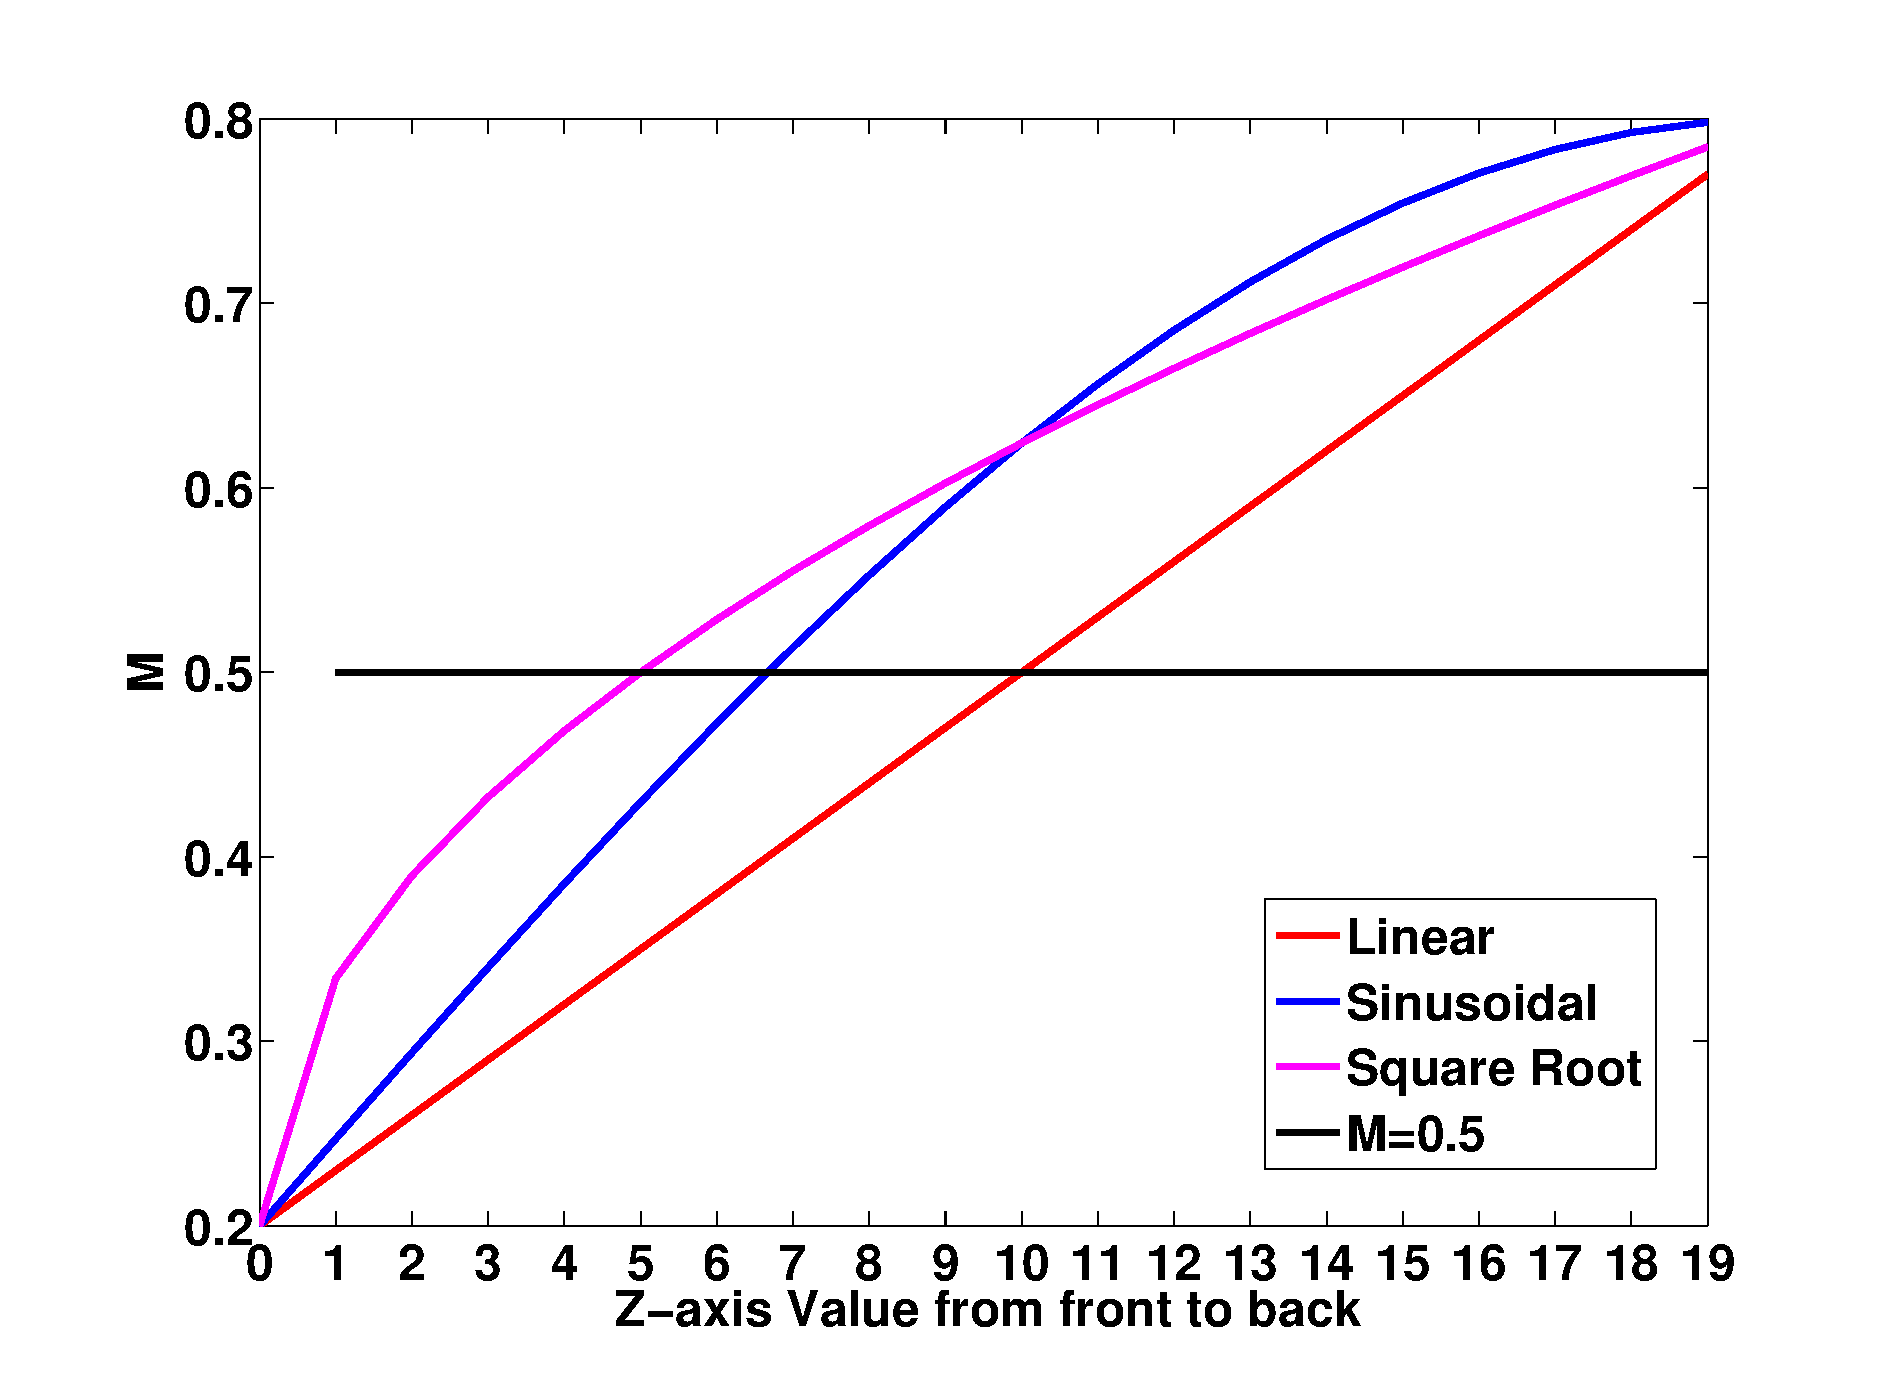
\includegraphics[width=0.6\textwidth]{fig_Results4_1.eps}
  \caption{Three functional forms of M variation comparison. They begin to exceed the M$=0.5$ black line at Z=10, 7, 5 for linear, sinusoidal and square root respectively.}
 \label{fig_Results4_1}
\end{figure}   

\paragraph{Secondary Fault}

For linear, the secondary fault at higher M side begins to take place at around 900kyrs (Figure~\ref{fig_Results4_2}), its spatial distribution is at M$>0.5$ region. It nucleates from the shear low (ridge center where M$=0.5$) to the M$=0.8$ end (Figure~\ref{fig_Results4_1} where the red line begin to exceeds 0.5 at Z$=10$). As it evolve, the initial detachment becomes inactive. This secondary fault creates another dome with initial composition likely to be volcanic rather than ultramafic, however, as it evolves, if it can last long enough to cut through the whole crust, mantle materials might exhume to the surface. The composition of the domes observed at Kane magamullions is similar to this mechanism between ultramafic babel dome and eastern to it the crustal inside-corner high. 

\begin{figure}[hc]
  \centering
    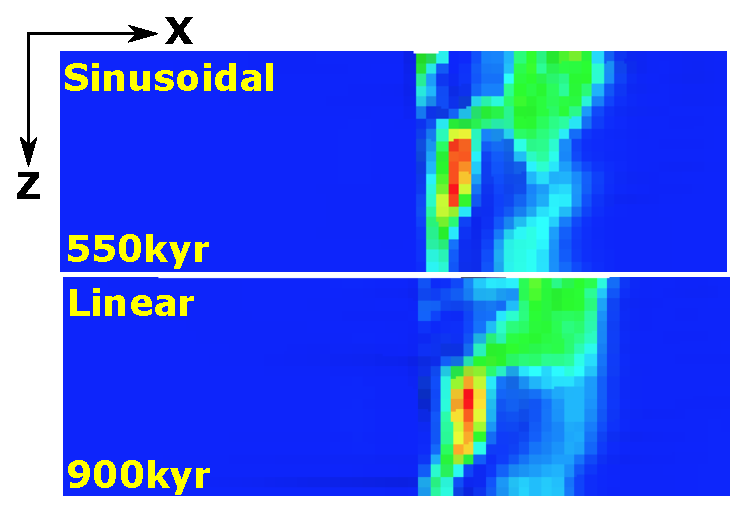
\includegraphics[width=0.6\textwidth]{fig_Results4_2_secondary_fault_length_comparison.eps}
  \caption{Secondary fault length comparison between linear and sinusoidal. Around 13 elements in length for sinusoidal compared to 11 elements for linear.}
 \label{fig_Results4_2}
\end{figure}   

For sinusoidal, the secondary fault begins to form at a much earlier time around 550kyrs (Figure~\ref{fig_Results4_2}), this is due to the total area above M$>0.5$ for sinusoidal functional form is higher than that of linear. Qualitatively, the total force to push the hanging wall of the detachment away from the dike for sinusoidal is higher than that of linear. Considering the mechanism for forming a secondary fault as mentioned in the ``Introduction'' section, the secondary fault should apear earlier in the sinusoidal functional form model. In addition, the total length of the secondary fault is longer due to the total length of M that is larger than 0.5 is bigger than that of the linear model (Figure~\ref{fig_Results4_1}). 
For square root, there is no secondary fault forming because the ``cut back'' behavior releases the tensional stress in the hanging wall.

\paragraph{Cut back behavior}

\begin{figure}[hc]
  \centering
    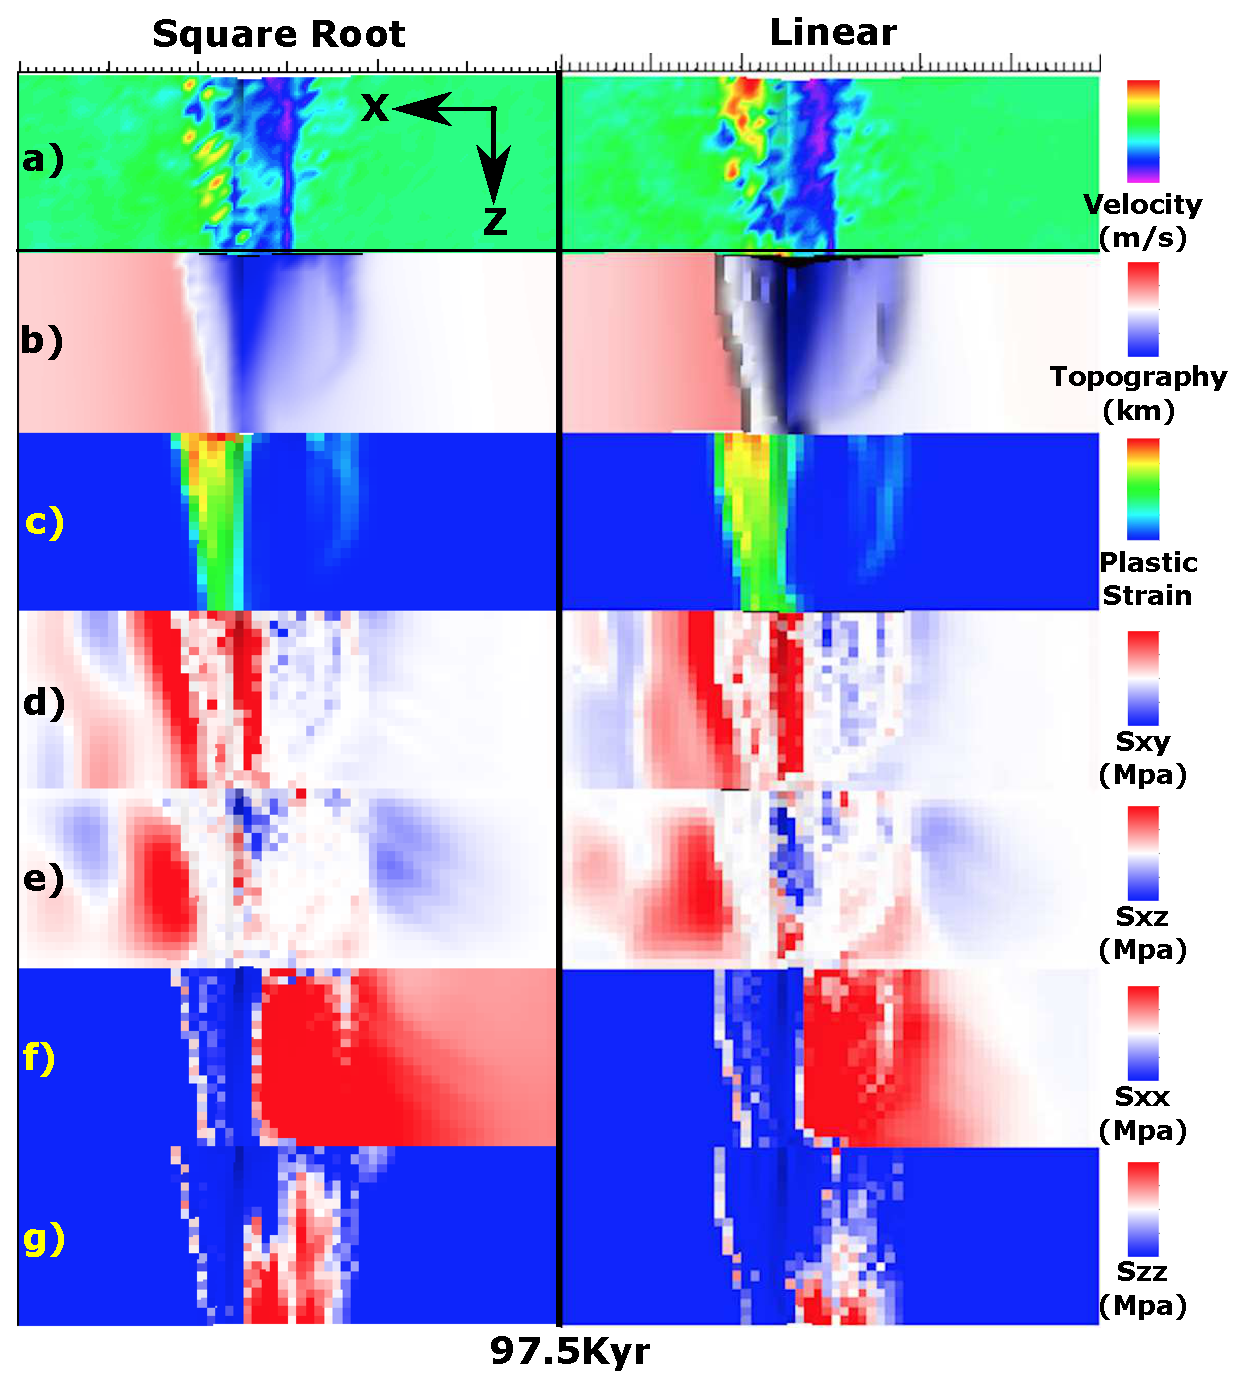
\includegraphics[width=0.6\textwidth]{fig_Results4_3_sqrt_vs_lin_cut_back_97kyr.eps}
  \caption{View from top of the model.}
 \label{fig_Results4_3_1}
\end{figure}  

\begin{figure}[hc]
  \centering
    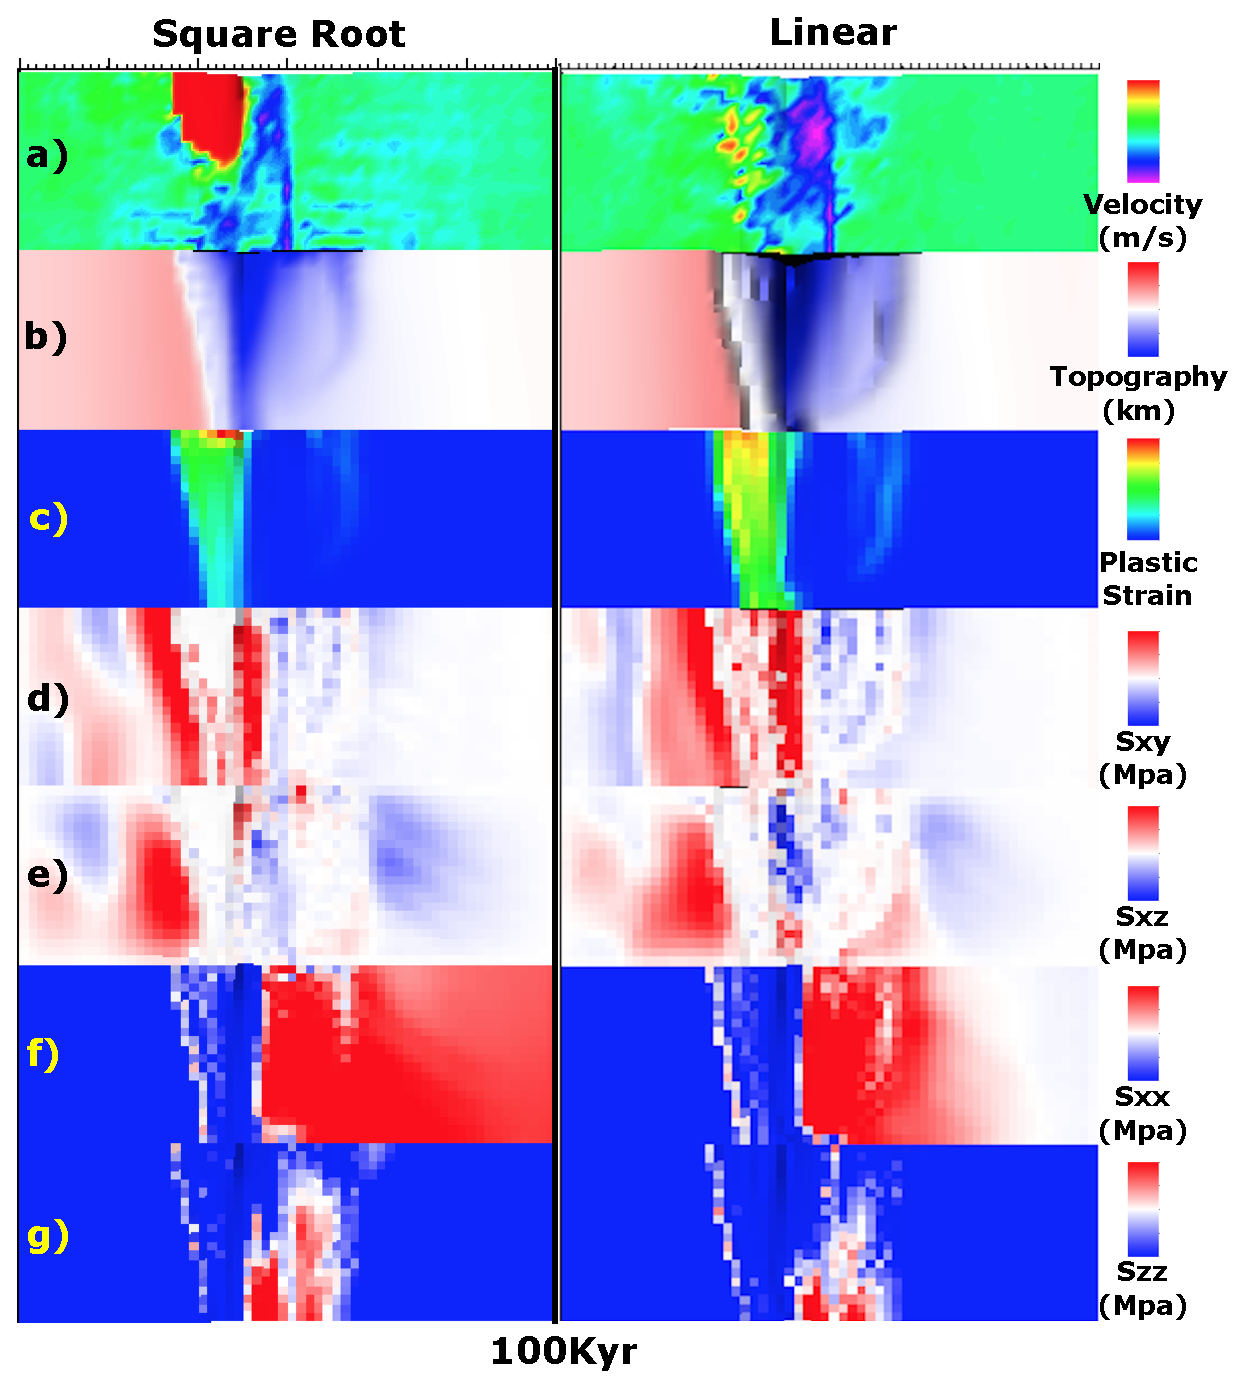
\includegraphics[width=0.6\textwidth]{fig_Results4_3_sqrt_vs_lin_cut_back_100kyr.eps}
  \caption{View from top of the model.}
 \label{fig_Results4_3_2}
\end{figure} 

The cut back happens mostly in the square root model. Since the linear model and the square root model have more obvious difference in terms of the cut back behavior, here, we only compare linear and square root. At the higher M side, the amount of diking for the square root model is ubiquitously larger than that of the linear one (Figure~\ref{fig_Results4_1}). This leads to a slower extending breakaway at the high M side for the square root model. However, at the low M side, due to higher value of $\frac{dM}{dZ}$ for square root, $\sigma_{xz}$ is focused at low Z ajacent to the ridge-axis (Figure~\ref{fig_Results4_3_1}.e), however for linear is spread out to Z higher than 10. The parallel to spreading direction offset between breakaways along the ridge-axis is 4km for square root compared to 3km for linear (Figure~\ref{fig_Results4_3_1}.c). Thus, the square root model experiences bigger shear force (both in $\sigma_{xz}$ and $\sigma_{xy}$) at the low M side and leads to the decouple of the hanging wall at the high M side as shown in Figure~\ref{fig_Results4_3_2}.a, the hanging wall is moving backwards to the dike in a high velocity with a suddenly drop at the tip of the breakaway at low M side (\add[XT]{this fault scarp behavior will be shown much obvious in the topography with different viewing angle (to be added) and even better at time 160kyr(must be added)}). 

     

\subsection{Variation of the range of M}
We have three ranges for M variation along the ridge-axis: M28, M57 and M58 (M28 means M varies from 0.2 to 0.8 from front to end as Z increases). One distinct difference between M58 and M57 or M28 is only models with range M58 produce fault alternation.

\subsection{Influence of weakening rate}
\citep{Lavier2000} shows higher characteristic fault offset result in more multiple fault. Only Type two weakening can produce alternating normal fault.
\subsection{Fault Alternation}
The fault alternation behavior observed in pseudo-2D models in cases M$>0.5$ is much more complicated in 3D models. The results shows that only Type two weakening with M58 will result in a alternating faulting pattern. \add[XT]{integrate the area of M$>0.5$ with respect to Z to see if there is any quantatative analysis available.}
\subsection{Corrugation}
The stress at the tips of the breakaways is generally tensional in both parallel and orthogonal directions to the ridge-axis. (Figure~\ref{fig_Results4_3_1}.f,g)
\subsection{Summary of Findings}
